\scanpage{16}
Polygône régulier (ou réalisation régulière d'un polygône combinatoire) : définitions possibles (cotés égaux, angles égaux,
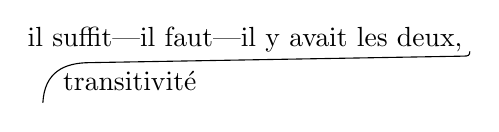
\begin{tikzpicture}[baseline=(trans.base)]
\node[anchor=base west,inner sep=0pt] (addtop) at (-.45,.55) {\inserted{\deleted{\unsure{il suffit|il faut|il y avait}} les deux,}};
\node[anchor=base west,inner sep=0pt] (trans) at (0,0) {transitivité};
\draw (-.25,-.16) .. controls (-.23,.23) and (.02,.35) .. (.35,.35)
 -- ([yshift=-.12em]addtop.south east) .. controls +(0.2em,0) and +(0,-.15em) .. ([xshift=.25em,yshift=.05em]addtop.south east);
\end{tikzpicture}
groupe des symétries ...) Existence,
\reversemarginpar
\margin{\figure{\begin{tikzpicture}[x=.8cm,y=.8cm]
\draw (0,0) -- (1.14,.66);
\draw (1.18,.70) -- (1.55,1.91);
\node[inner sep=0pt] at (.68,1.19) {$\unsure{.}$};
\end{tikzpicture}}}
\normalmarginpar
unicité modulo homothétie : tout isom. combinatoire est induit par une unique similitude.

Notion d'enveloppe affine (ou vectorielle) d'un polygône combinatoire ... \unsure{sens|sans} précisé

\noindent Fonctorialité de
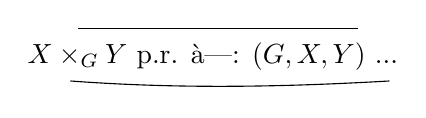
\begin{tikzpicture}[baseline=(fun.base)]
\node[anchor=base west,inner sep=0pt] (fun) at (0,0) {$X\times_G Y$ p.r. \unsure{à|:} $(G,X,Y)$ ...};
\draw (.65,.45) -- (4.2,.45);
\draw (.55,-.22) .. controls (1.9,-.32) and (3.2,-.30) .. (4.6,-.22);
\end{tikzpicture}

\[
\unsure{P|\overline{P}}\times_G E={}^{P}\!\deleted{B}E=F
\qquad\qquad
\begin{array}{ll}
P&G\text{-torseur}\\[.3em]
E&G\text{-ensemble}
\end{array}
\]

$P\longrightarrow\operatorname{Bij}(E,F)$ compatible aux opérations de $G$ à droite

\uline{NB} Si $G$ opère fidèlement sur $E$, $G$ opère ``sans pts fixes'' sur $\operatorname{Bij}(E,F)$ --- i.e. $\deleted{\unsure{y}}\unsure{x|y|u}.g=\unsure{u|x}$ $(g\in G,\ x\in B)$ implique $g=1$, ou encore les $G_x$ $(x\in B)$ sont réduits à $\{1\}$, ou encore $B$ est une somme de torseurs ... Dans ce cas
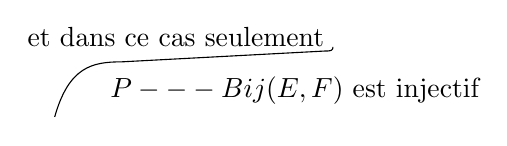
\begin{tikzpicture}[baseline=(injtext.base)]
\node[anchor=base west,inner sep=0pt] (addcase) at (0,.64) {\inserted{et dans ce cas seulement}};
\node[anchor=base west,inner sep=0pt] (injtext) at (1.05,0) {$P\mathbin{\text{---}}\operatorname{Bij}(E,F)$ est injectif};
\draw (.35,-.25) .. controls (.53,.39) and (.83,.45) .. (1.20,.45)
 -- ([yshift=-.13em]addcase.south east) .. controls +(.25em,0) and +(0,-.13em) .. ([xshift=.3em,yshift=.02em]addcase.south east);
\end{tikzpicture}

\[
P\hookrightarrow\operatorname{Bij}(E,F)
\]

% slanted; left margin, rising to the right
\reversemarginpar
\margin{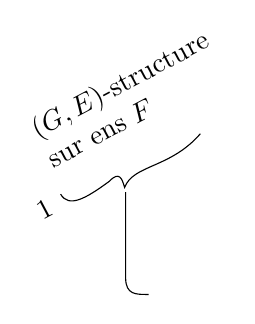
\begin{tikzpicture}[x=.65cm,y=.65cm,baseline=(side.base)]
\node[anchor=base west,inner sep=0pt,rotate=28] (side) at (-.25,.8) {\shortstack[l]{$(G,E)$-structure\\sur ens $F$}};
\draw (-.10,.30) .. controls (.06,.02) and (.40,.22) .. (.85,.55)
 .. controls (1.05,.76) and (1.10,.60) .. (1.15,.43)
 .. controls (1.32,.88) and (2.04,.80) .. (2.63,1.48);
\node[anchor=base west,inner sep=0pt,rotate=28] at (-.46,-.22) {\deleted{\illegible{1}}};
\draw (1.17,.34) -- (1.17,-1.33) .. controls (1.17,-1.67) and (1.37,-1.66) .. (1.62,-1.66);
\end{tikzpicture}}
\normalmarginpar
\noindent$\left[\begin{minipage}{.84\linewidth}
En tous les cas,
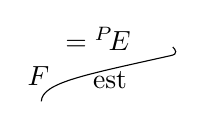
\begin{tikzpicture}[baseline=(fbase.base)]
\node[anchor=base west,inner sep=0pt] (fbase) at (0,0) {$F$};
\node[anchor=base west,inner sep=0pt] at (.48,.44) {$\inserted{={}^{P}\!E}$};
\node[anchor=base west,inner sep=0pt] at (.83,-.04) {est};
\draw (.18,-.20) .. controls (.19,.04) and (.75,.14) .. (1.82,.38)
 .. controls (1.93,.40) and (1.88,.46) .. (1.85,.49);
\end{tikzpicture}
muni de la structure suivante : donnée d'une orbite de $G$ dans $\operatorname{Bij}(E,F)$.
\end{minipage}\right.$

% The small right-hand note overlaps the larger Corollaire baseline below it.
\noindent\begin{tikzpicture}
\node[anchor=north west,inner sep=0pt,text width=.66\linewidth,font=\footnotesize] at (.34\linewidth,0) {[On verra que (si $G$ opère $\unsure{\text{fid}^{\mathrm{t}}}$ sur $E$) la donnée d'un
\begin{tikzpicture}[baseline=(oldlower.base)]
\node[anchor=base west,inner sep=0pt] at (0,.27) {\deleted{\unsure{ens|d'un}}};
\node[anchor=base west,inner sep=0pt] (oldlower) at (0,0) {\deleted{\unsure{$(G,E)$-st}}};
\end{tikzpicture}
$F$ avec $(G,E)$-structure \unsure{équivaut à|équiv. à} \unsure{celle d'un} \unsure{$G$-torseur} \unsure{et applic$^{\mathrm{tn}}$}.]};
\node[anchor=north west,inner sep=0pt,text width=.54\linewidth] at (.46\linewidth,-1.65) {\uline{Corollaire} \unsure{de|du} $\big[\,\unsure{.}\,\unsure{\mathbin{\text{---}}|\longrightarrow}$ \unsure{toute structure}};
\end{tikzpicture}
% archive sheet number: 15
